\documentclass[12pt]{article}

\usepackage[a4paper,margin=2.5cm]{geometry}
\usepackage{amsmath, amssymb, amsthm}
\usepackage{bm}
\usepackage{hyperref}
\usepackage{graphicx}
\usepackage{caption}
\usepackage{listings}
\usepackage{xcolor}
\usepackage{float}
\usepackage{placeins}
\graphicspath{{figures/}}

\lstdefinestyle{code}{
  basicstyle=\ttfamily\small,
  numbers=left,
  numberstyle=\tiny,
  numbersep=8pt,
  keywordstyle=\color{blue},
  commentstyle=\color{teal!70!black},
  stringstyle=\color{orange!70!black},
  showstringspaces=false,
  breaklines=true,
  frame=single,
  framerule=0.3pt,
  rulecolor=\color{black!15}
}
\lstset{style=code}

\title{Policy Gradient Methods Tutorial}
\author{}
\date{\today}

\begin{document}
\maketitle

\section{Introduction}
Policy gradient methods directly optimize a parameterized policy by ascending the gradient of expected return. Unlike value-based methods that derive policies from action-value estimates, policy gradients handle continuous action spaces, stochastic policies, and incorporate constraints such as entropy regularization with ease.

\section{Theory and Formulas}
\subsection{Objective and Policy Gradient Theorem}
Let a stochastic policy \(\pi_\theta(a\mid s)\) be parameterized by \(\theta\). The objective is the expected discounted return
\begin{equation}
J(\theta) = \mathbb{E}_{\tau \sim \pi_\theta}\Big[ \sum_{t=0}^{T} \gamma^t r_{t+1} \Big],
\end{equation}
where \(\tau\) denotes trajectories sampled under \(\pi_\theta\). The policy gradient theorem states
\begin{equation}
\nabla_\theta J(\theta) = \mathbb{E}_{s \sim d^{\pi_\theta}, a \sim \pi_\theta}\big[ \nabla_\theta \log \pi_\theta(a\mid s)\, Q^{\pi_\theta}(s,a) \big],
\end{equation}
with \(d^{\pi_\theta}\) the discounted state visitation distribution.

\subsection{Baselines and Advantage Estimates}
To reduce variance, a baseline \(b(s)\) can be subtracted without bias:
\begin{equation}
\nabla_\theta J(\theta) = \mathbb{E}\big[ \nabla_\theta \log \pi_\theta(a\mid s)\, (Q^{\pi}(s,a) - b(s)) \big].
\end{equation}
Choosing \(b(s)=V^{\pi}(s)\) yields the advantage function \(A^{\pi}(s,a)\), motivating actor-critic architectures where a value estimator supplies the baseline.

\subsection{Update Rule}
Monte Carlo policy gradient performs stochastic ascent:
\begin{equation}
\theta_{k+1} = \theta_k + \alpha \sum_{t=0}^{T-1} \nabla_\theta \log \pi_{\theta_k}(a_t\mid s_t)\, \hat{A}_t,
\end{equation}
where \(\hat{A}_t\) is an estimator of the advantage (returns, generalized advantage estimation, etc.). Learning rates \(\alpha\), gradient clipping, and entropy bonuses stabilize optimization.

\section{Applications and Tips}
\begin{itemize}
  \item \textbf{Continuous control}: robotics, locomotion, and control tasks with continuous actions (e.g., PPO, TRPO variants).
  \item \textbf{Constrained optimization}: incorporate safety constraints via penalty or Lagrangian formulations while still using gradients.
  \item \textbf{Imitation and fine-tuning}: initialize from expert demonstrations and refine via policy gradients.
  \item \textbf{Best practices}: normalize advantages, use adaptive optimizers (Adam), maintain entropy regularization, and monitor gradient norms.
\end{itemize}

\section{Python Practice}
The script \texttt{gen\_policy\_gradient\_figures.py} trains a softmax policy on a stochastic bandit-style environment using REINFORCE with a learned baseline. It logs episode returns and gradient norms to visualize learning stability.
\begin{lstlisting}[language=Python,caption={Excerpt from gen_policy_gradient_figures.py}]
grad = features[action] - (policy @ features)
baseline = baseline + baseline_lr * (G - baseline)
theta += alpha * grad * (G - baseline)
\end{lstlisting}

\section{Result}
\begin{figure}[H]
  \centering
  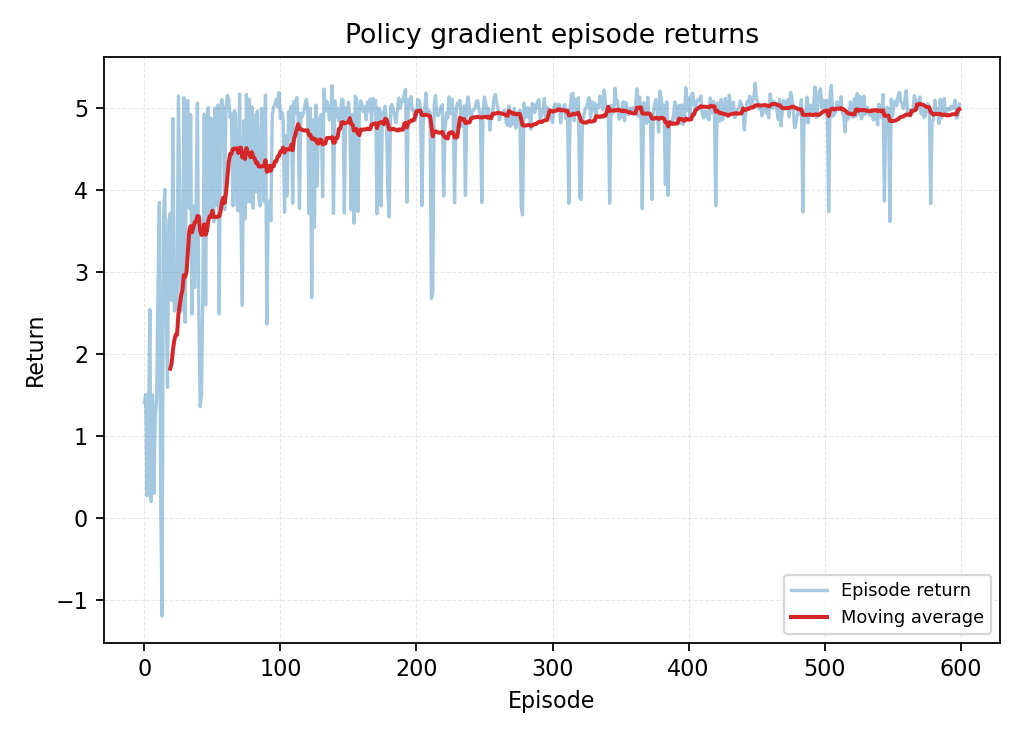
\includegraphics[width=0.8\linewidth]{policy_gradient_returns.png}
  \caption{Policy gradient episode returns with moving average smoothing}
  \label{fig:policy_gradient_returns}
\end{figure}

\begin{figure}[H]
  \centering
  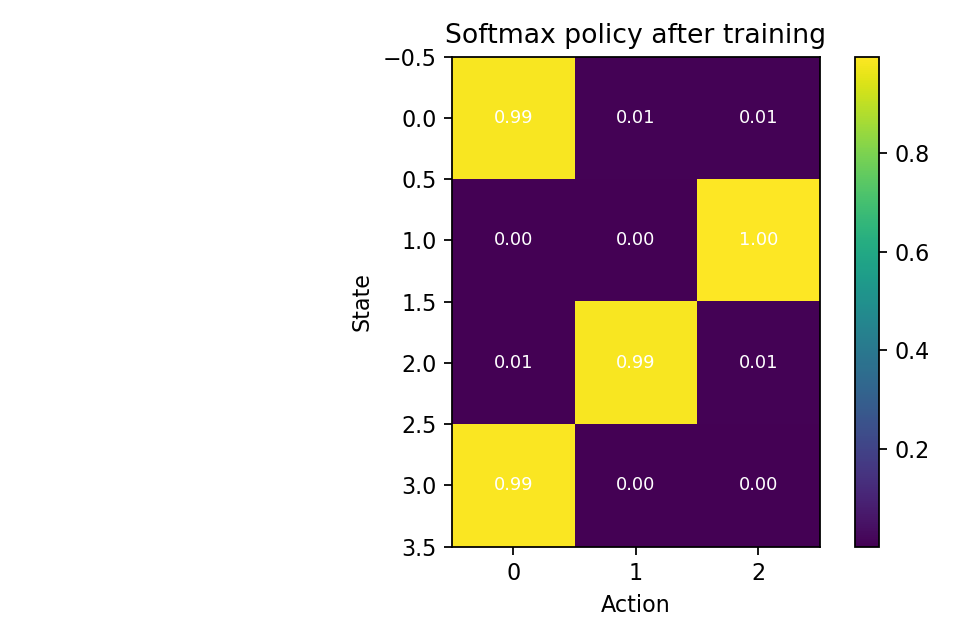
\includegraphics[width=0.82\linewidth]{policy_gradient_policy_heatmap.png}
  \caption{State-action probability heatmap learned by the softmax policy}
  \label{fig:policy_gradient_policy_heatmap}
\end{figure}

\FloatBarrier
\section{Summary}
Policy gradients provide a principled way to optimize stochastic policies through gradient ascent on expected returns. Variance reduction, entropy bonuses, and adaptive optimizers are crucial for stable training. The bandit example highlights how returns improve and how the policy distribution sharpens toward high-reward actions.

\end{document}